\documentclass[11pt,a4paper]{article}
\usepackage[T1]{fontenc}\usepackage{lmodern}\usepackage[scaled=0.92]{helvet}
\usepackage[margin=2.2cm]{geometry}
\usepackage{amsmath,amssymb,booktabs,array,tabularx,graphicx,xcolor,enumitem,tikz}
\usetikzlibrary{positioning,arrows.meta,calc,fit,backgrounds,shapes.geometric}
\definecolor{mechblue}{HTML}{2A78D6}\definecolor{advorange}{HTML}{C9541F}\definecolor{okgreen}{HTML}{0E7C4F}
\usepackage{xr-hyper}\externaldocument{../manuscript/main}
\usepackage[hidelinks]{hyperref}
\usepackage[most]{tcolorbox}
\usepackage{titlesec}
\titleformat{\section}{\sffamily\Large\bfseries\color{mechblue!80!black}}{\thesection}{0.6em}{}
\titleformat{\subsection}{\sffamily\large\bfseries}{\thesubsection}{0.5em}{}
\setlength{\parindent}{0pt}\setlength{\parskip}{0.55em}
\setlist{itemsep=0.15em,topsep=0.3em}
\newtcolorbox{analogy}[1][]{colback=okgreen!6,colframe=okgreen!70!black,fonttitle=\sffamily\bfseries,title={In everyday terms#1},boxrule=0.6pt,arc=2pt}
\newtcolorbox{keypoint}[1][]{colback=mechblue!6,colframe=mechblue!80!black,fonttitle=\sffamily\bfseries,title={#1},boxrule=0.6pt,arc=2pt}
\newtcolorbox{caution}[1][]{colback=advorange!6,colframe=advorange!80!black,fonttitle=\sffamily\bfseries,title={#1},boxrule=0.6pt,arc=2pt}
\newcommand{\mech}[1]{\textsf{\textcolor{mechblue!80!black}{#1}}}
\newcommand{\adv}[1]{\textsf{\textcolor{advorange!85!black}{#1}}}
\newcommand{\cmd}[1]{\texttt{\small #1}}

\title{\sffamily\bfseries How the Experiments Were Conducted\\[2pt]
\large\mdseries Procedure guide for \emph{What Can Provenance Prove?} (manuscript v12)}
\author{Waqas Ahmed \and Ammar Hassan \and Attiq Ahmed \and Waseem Iqbal}
\date{21 November 2026}
\begin{document}
\sloppy
\maketitle

\begin{keypoint}{What this guide is}
A step-by-step record of every check and experiment in the paper: what question it answers,
what was run, on which machine, how the results were validated, and where the raw files are.
It is written so that a reader can repeat any experiment. Every number below is the one in the
manuscript; none was typed into the paper by hand (tables are generated by scripts from raw
result files).
\end{keypoint}

\tableofcontents

\section{The plan in one picture}

The paper makes exact claims about a mathematical model, then tests whether real systems
behave as the model says. The work therefore has three layers (Fig.~\ref{fig:plan}).

\begin{figure}[h]
\centering
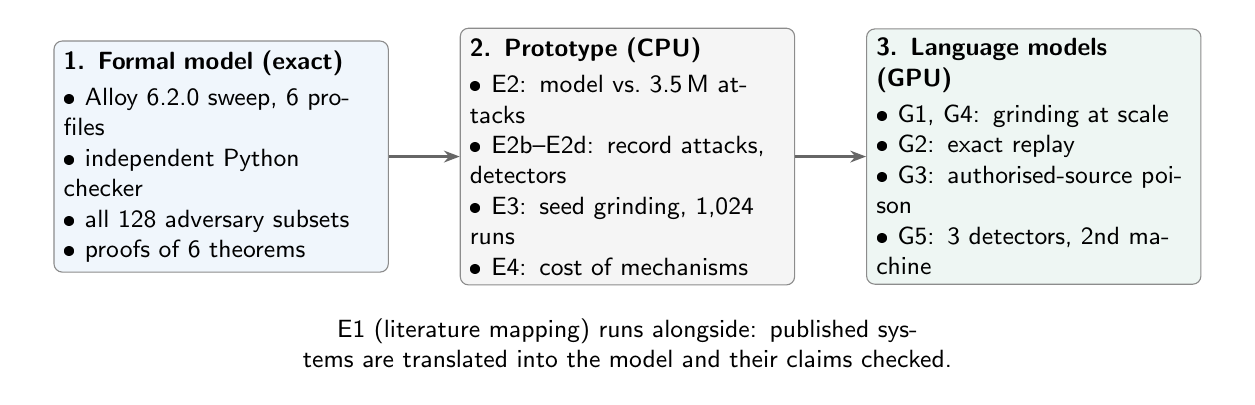
\begin{tikzpicture}[font=\sffamily\small, >={Stealth[length=2mm]},
  lay/.style={draw=black!45, rounded corners=3pt, fill=#1, text width=40mm, align=left, inner sep=3.5pt, minimum height=27mm},
  hd/.style={font=\sffamily\bfseries}, fl/.style={->, black!60, line width=0.9pt}]
\node[lay=mechblue!7] (a) at (0,0) {{\bfseries 1. Formal model (exact)}\\[2pt]
  \textbullet\ Alloy 6.2.0 sweep, 6 profiles\\ \textbullet\ independent Python checker\\
  \textbullet\ all 128 adversary subsets\\ \textbullet\ proofs of 6 theorems};
\node[lay=black!4, right=9mm of a] (b) {{\bfseries 2. Prototype (CPU)}\\[2pt]
  \textbullet\ E2: model vs.\ 3.5\,M attacks\\ \textbullet\ E2b--E2d: record attacks, detectors\\
  \textbullet\ E3: seed grinding, 1,024 runs\\ \textbullet\ E4: cost of mechanisms};
\node[lay=okgreen!7, right=9mm of b] (c) {{\bfseries 3. Language models (GPU)}\\[2pt]
  \textbullet\ G1, G4: grinding at scale\\ \textbullet\ G2: exact replay\\
  \textbullet\ G3: authorised-source poison\\ \textbullet\ G5: 3 detectors, 2nd machine};
\draw[fl] (a) -- (b);
\draw[fl] (b) -- (c);
\node[below=3mm of b, text width=150mm, align=center, font=\sffamily\small] {E1 (literature mapping) runs alongside: published systems are translated into the model and their claims checked.};
\end{tikzpicture}
\caption{The three layers of evidence. The model predicts; the prototype tests the predictions; the GPU experiments test them at language-model scale.}\label{fig:plan}
\end{figure}

\begin{center}\small
\begin{tabularx}{\textwidth}{@{}l>{\raggedright}X>{\raggedright}X>{\raggedright\arraybackslash}X@{}}
\toprule
ID & Question & Set-up & Machine\\
\midrule
Model & For which mechanism sets is a goal guaranteed? & Alloy sweep; independent checker; 128-subset lattice & cloud workspace (CPU)\\
E1 & What do published systems actually guarantee? & each paper's mechanisms mapped to the model & desk study\\
E2 & Do real executions match the model? & prototype pipeline, adaptive attacker, 9,216 instances & cloud workspace (CPU)\\
E2b & Do record-level attacks behave as predicted? & split view, equivocation, censorship & cloud workspace (CPU)\\
E2c/E2d & What do detectors catch when poison has valid receipts? & 0--100 poisoned items, 1--3 detectors & cloud workspace (CPU)\\
E3 & How much can a prover steer a model by choosing seeds? & 1,024 training runs & cloud workspace (CPU)\\
E4 & What do the record mechanisms cost? & 1k--100k items, one core & cloud workspace (CPU)\\
G1, G4 & Does grinding work on real language models? & DistilBERT (160 runs); Qwen2.5-0.5B + LoRA (48 runs) & RTX 3070 laptop\\
G2 & Does re-training reproduce the same model? & 3 runs per configuration & RTX 3070 laptop\\
G3 & Does provenance stop authorised-source poison? & DistilBERT, SST-2, 0--160 poisoned & RTX 3070 laptop\\
G5 & Three detectors, a clean baseline, higher poison; replay on another GPU & DistilBERT, SST-2, 0--320 poisoned & GTX 1650 desktop\\
\bottomrule
\end{tabularx}
\end{center}

\section{Rules followed in every experiment}
\begin{enumerate}
\item \textbf{Fixed seeds.} Every random choice uses a recorded seed, so a run can be repeated.
\item \textbf{Raw files are never edited.} Each experiment writes its raw output once. Analysis
  scripts only read them. A re-run never overwrites an earlier run (it is renamed).
\item \textbf{No hand-typed numbers.} Tables and numbers in the paper are generated by scripts
  (\cmd{make\_tables.py}, \cmd{stats\_revision.py}, \cmd{make\_e2d\_rows.py},
  \cmd{make\_g5\_tables.py}) from the raw files.
\item \textbf{Rules fixed before results.} Detector flagging rules, analysis methods and
  validation checks were written before the run they apply to (for G5, before it ran).
\item \textbf{Honest scope.} The trusted hardware in the prototype is \emph{simulated}; model
  checking is exact for the model at the stated scope, not a statement about deployed systems.
\item \textbf{Who ran what.} The formal checks, the prototype experiments (E2--E4) and all
  analyses ran in Claude's cloud workspace. The GPU experiments ran on the authors' own
  machines, started by the first author; the result files were then read and checked.
\end{enumerate}

\section{The formal model checks}
\subsection*{Procedure}
\begin{enumerate}
\item \textbf{Write the model.} The pipeline (sources, generator, transform, capture,
  executor), the seven mechanisms and the seven adversary capabilities are written in Alloy
  (\cmd{model\_v3/pipeline\_v3\_base.als}).
\item \textbf{Sweep.} \cmd{model\_v3/sweep.py} asks Alloy, for each of 6 adversary profiles
  $\times$ 2 pipeline types $\times$ 128 mechanism sets $\times$ 6 goals (9,216 instances), whether
  an accepted execution can violate the goal. Scope 5 (up to 5 items).
\item \textbf{Check independently.} \cmd{model\_v3/independent\_check.py} decides the same
  9,216 instances by a different method (exhaustive enumeration of single-item executions,
  justified by the separability lemma). Both methods must agree on every instance; they do.
\item \textbf{All adversaries.} \cmd{lattice/adversary\_lattice.py} repeats the decision for all
  $2^7=128$ adversary capability subsets (196,608 decisions), and
  \cmd{check\_theorems\_on\_lattice.py} checks every theorem against every decision.
\item \textbf{Prove.} The theorems are proved by hand (Supplementary Section S10). When a
  check disagreed with a draft theorem, the theorem was corrected (this happened for
  Theorem~1, whose extra assumption was removed, and led to Corollary~1).
\end{enumerate}

\section{The prototype experiments (E2--E4)}
\subsection{The prototype}
A small but real pipeline in Python: four authorised sources sign 1,500 movie reviews
(polarity dataset v2.0) with Ed25519 keys; a generator adds 150 synthetic reviews; a
transform filters short and duplicate reviews; capture commits a Merkle root to a
transparency log with co-signing witnesses; the executor trains a small bag-of-words network
deterministically on CPU. Each mechanism is implemented (binding by exact re-execution, signed
receipts, input witness, simulated enclave, spectral detector).

\subsection{E2: does reality match the model?}
\begin{enumerate}
\item For each of the 9,216 instances, build the pipeline with that mechanism set.
\item Let the adversary run \emph{every subset} of the attacks it is allowed (inject, launder,
  omit, reinstate, hide poison, grind the seed, collude, extract enclave keys), with 1 and 8
  poisoned items.
\item Apply the auditor's checks; for accepted executions, test the six goals on the
  recorded ground truth.
\item Compare with the model: a \emph{soundness failure} is an accepted execution that breaks
  a goal the model guarantees; a \emph{realised failure} is a predicted failure shown by a
  real attack.
\end{enumerate}
Result: 3,498,118 executions, 656,798 accepted, \textbf{0} soundness failures, and all
\textbf{4,440} predicted failures realised. The first sweep missed 20; the model's
counterexamples pointed to two attacks we had not implemented, which closed the gap.

\subsection{E2b--E2d: records and detectors}
\begin{itemize}
\item \textbf{E2b split view:} a source signs a clean review and serves a poisoned one under the
  same name. Name-only receipts accepted 200/200; content-addressed receipts 0/200.
\item \textbf{E2b equivocation and censorship:} a log operator signs two different histories
  (caught by the witness) or silently drops an entry (not caught: 20/20 heads co-signed).
\item \textbf{E2c:} 0--100 poisoned items with valid receipts; attack success and the spectral
  detector's recall, 3 seeds each.
\item \textbf{E2d:} adds a clean baseline and two more detectors (activation clustering, loss).
\end{itemize}

\subsection{E3: seed grinding}
\begin{enumerate}
\item Train the same model on the same committed data 1,024 times, changing only the seed.
  Check that re-running a seed gives identical weights.
\item Split runs into 128 \emph{selection} runs (to pick sensitive test inputs, ``probes'') and
  896 \emph{evaluation} runs.
\item For each target pattern of $k$ probe predictions and each budget of $T$ runs, compute
  exactly the probability that one of $T$ runs produces the pattern.
\item Report the largest $k$ reached with probability $\ge 1/2$. Result: exactly $\log_2 T$
  bits (9 bits at $T=512$), matching Theorem~4.
\end{enumerate}

\subsection{E4: cost}
Hashing, signing and verifying receipts, and computing Merkle roots for 1,000, 10,000 and
100,000 items on one CPU core. Verifying a receipt takes about 116--155\,\textmu s.

\section{The GPU experiments (G1--G5)}
\subsection{Common set-up}
SST-2 sentiment data (GLUE) and two models: DistilBERT (full fine-tuning) and Qwen2.5-0.5B
with LoRA (rank 8). One epoch, bf16 mixed precision, maximum length 64, deterministic GPU
kernels. The kit (\cmd{p3gpu.py}, \cmd{run\_gpu.ps1}) creates a private Python environment
and records versions and a log.

\begin{center}\small
\begin{tabular}{@{}lll@{}}
\toprule
& G1--G4 & G5\\
\midrule
Machine & RTX 3070 Laptop GPU, 8\,GB & GTX 1650, 4\,GB (desktop)\\
Software & Python 3.11.9, PyTorch 2.6.0+cu124 & Python 3.14.10, PyTorch 2.11.0+cu128\\
Shared & \multicolumn{2}{l}{Transformers 5.22.1, PEFT 0.21.2, datasets 5.1.0}\\
\bottomrule
\end{tabular}
\end{center}

\subsection{G1--G4}
\begin{itemize}
\item \textbf{G2 replay:} train 3 times with the same seed on 1,000 examples, deterministic and
  default kernels, both models; compare weight hashes. Result: identical in all cases.
\item \textbf{G3 poison:} add 0, 20, 40, 80 or 160 poisoned examples (trigger ``cf'', negative
  sentences relabelled positive) to 8,000 clean ones, all with valid signed receipts; train 3
  seeds each; measure attack success, clean accuracy and spectral-signature recall.
\item \textbf{G1/G4 grinding:} 160 DistilBERT runs and 48 Qwen+LoRA runs on fixed data, analysed
  exactly like E3. Result: $\log_2 T$ bits (7 bits at $T=128$; 5 bits at $T=32$).
\end{itemize}

\subsection{G5, step by step}
\begin{figure}[h]
\centering
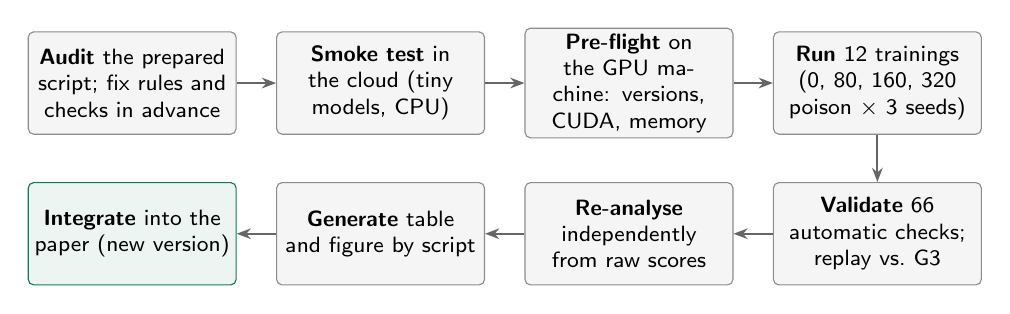
\begin{tikzpicture}[font=\sffamily\footnotesize, >={Stealth[length=1.8mm]},
  s/.style={draw=black!45, rounded corners=2pt, fill=black!4, text width=25mm, align=center, minimum height=13mm, inner sep=2pt},
  fl/.style={->, black!60, line width=0.8pt}]
\node[s] (1) {\textbf{Audit} the prepared script; fix rules and checks in advance};
\node[s, right=5mm of 1] (2) {\textbf{Smoke test} in the cloud (tiny models, CPU)};
\node[s, right=5mm of 2] (3) {\textbf{Pre-flight} on the GPU machine: versions, CUDA, memory};
\node[s, right=5mm of 3] (4) {\textbf{Run} 12 trainings (0, 80, 160, 320 poison $\times$ 3 seeds)};
\node[s, below=6mm of 4] (5) {\textbf{Validate} 66 automatic checks; replay vs.\ G3};
\node[s, left=5mm of 5] (6) {\textbf{Re-analyse} independently from raw scores};
\node[s, left=5mm of 6] (7) {\textbf{Generate} table and figure by script};
\node[s, left=5mm of 7, fill=okgreen!8, draw=okgreen] (8) {\textbf{Integrate} into the paper (new version)};
\draw[fl] (1)--(2); \draw[fl] (2)--(3); \draw[fl] (3)--(4); \draw[fl] (4)--(5); \draw[fl] (5)--(6); \draw[fl] (6)--(7); \draw[fl] (7)--(8);
\end{tikzpicture}
\caption{The G5 procedure.}
\end{figure}

\begin{enumerate}
\item \textbf{Audit.} The prepared script was read in full. Two things were added before the
  run: the analysis script with the flagging rules of E2d (spectral and loss flag the top
  7.5\% per class; activation clustering flags a cluster smaller than 35\%), and 66 validation
  checks. The k-means iteration cap was aligned with E2d (100). Nothing that affects training
  was changed.
\item \textbf{Smoke test.} The whole pipeline ran in the cloud with tiny random models to show
  the code works. These outputs are not results.
\item \textbf{Set-up on the GPU machine.} The RTX 3070 was unavailable, so G5 ran on a desktop
  with a GTX 1650. The first set-up attempt failed because of a Python-detection bug in the
  set-up script; it was fixed and the second attempt succeeded. Pre-flight: all checks PASS,
  one warning (newer PyTorch).
\item \textbf{Run.} The first author double-clicked \cmd{START\_G5.bat}. 12 trainings,
  38 minutes, about 104\,s of training each, at most 1.4\,GB of GPU memory, all on CUDA with
  deterministic kernels. Every per-item detector score was saved.
\item \textbf{Validate.} 64 of 66 checks passed. The two failures were expected: the device is
  not the RTX 3070, and the 9 runs that repeat G3 did not reproduce G3 bit for bit (different
  GPU and software). This second ``failure'' is itself a finding: exact replay needs the same
  hardware and software.
\item \textbf{Re-analyse.} The analysis was re-run in the cloud from the raw files and gave
  identical results.
\item \textbf{Generate.} \cmd{make\_g5\_tables.py} and \cmd{fig\_g5.py} produce the paper's Table~\ref{tab:g5} and Fig.~\ref{fig:g5} from the raw analysis.
\item \textbf{Integrate.} New manuscript version; earlier versions kept.
\end{enumerate}

\subsection*{G5 results}
\begin{center}\small
\begin{tabular}{@{}rrrrr@{}}
\toprule
Poison & Attack success & Spectral recall (AUROC) & Loss recall (AUROC) & Act.\ clust.\ (clean)\\
\midrule
0\% & 13\% & -- & -- & flags 27\%\\
1.0\% & 17\% & 170/240 (0.90) & 172/240 (0.94) & flags 30\%\\
2.0\% & 52\% & 140/480 (0.66) & 136/480 (0.82) & flags 28\%\\
3.8\% & 100\% & 1/960 (0.44) & 1/960 (0.41) & flags 31\%\\
\bottomrule
\end{tabular}
\end{center}
AUROC measures how well a detector separates poisoned from clean items (1 = perfect,
0.5 = chance). Detection works only while the attack does not.

\section{How to repeat the experiments}
{\footnotesize
\begin{tabularx}{\textwidth}{@{}p{30mm}X@{}}
\toprule
Formal checks & \cmd{cd model\_v3}; \cmd{python sweep.py 5}; \cmd{python independent\_check.py 5}\\
& \cmd{cd lattice}; \cmd{python adversary\_lattice.py}; \cmd{python check\_theorems\_on\_lattice.py}\\
Prototype & \cmd{python exp/e2\_sweep.py full full+wit full+tee cap-only exec-only trans-only}\\
& \cmd{python exp/e2b\_targeted.py}; \cmd{python exp/e2c\_detector.py}; \cmd{python exp/e2d\_detectors.py}\\
& \cmd{python exp/e3\_grind.py 1024}; \cmd{python exp/e4\_overhead.py}\\
G1--G4 (Windows GPU) & \cmd{powershell -ExecutionPolicy Bypass -File .\textbackslash run\_gpu.ps1}\\
G5 (Windows GPU) & double-click \cmd{START\_G5.bat}, or run \cmd{g5\_preflight.py}, \cmd{p3gpu\_g5.py}, \cmd{g5\_analyse.py}\\
Tables and figures & \cmd{python exp/make\_tables.py}; \cmd{python exp/stats\_revision.py}; \cmd{python g5/make\_g5\_tables.py}; \cmd{python g5/fig\_g5.py}\\
\bottomrule
\end{tabularx}}

Full details, including the mapping from every table to its script and raw file, are in
\cmd{REPRODUCIBILITY.md} of the artefact (Zenodo DOI 10.5281/zenodo.24317967) and the GitHub
repository \cmd{waqas6755/what-can-provenance-prove}.

\section{Limits to keep in mind}
\begin{itemize}
\item The enclave in the prototype is simulated, not real trusted hardware.
\item Poisoning experiments use one model family (DistilBERT), one dataset, one trigger and
  three seeds per condition; they are reported descriptively.
\item Exact replay holds on one fixed machine and software stack, not across machines.
\item Experiments cover fine-tuning, not pre-training.
\item The literature screening was done by an AI assistant and still needs human screening.
\end{itemize}
\end{document}
